\documentclass{article}
\usepackage{setspace}
\usepackage[margin=1 in]{geometry}
\usepackage{amsmath,graphicx}
\author{\#Authors}
\title{Stereo odometry based on  Local Intensity Order Pattern}
\doublespacing
\begin{document}
\maketitle
\begin{abstract}
New generation autonomous vehicles use different data fusion techniques to solve the Simultaneous Localization And Mapping (SLAM) problems in urban terrains.  However, the majority of the implementations uses high-cost sensors like LIDAR to obtain a high accuracy map. In this paper, we  present a novel method  to solve this problem using sequences of stereo images. Our approach uses Local Intensity Order Pattern (LIOP) based  feature descriptors to  overcome the problem of monotonic intensity changes and affine transformations of detected features. Egomotion of the vehicle is estimated using correspondence of features on the consecutive frames. Estimated motion parameters are then corrected using an extended Kalman filter. Depth of the detected features is calculated using stereo triangulation. Mahalanobis distance  is used to avoid outliers in the detected features.
The accuracy of  the proposed method is  evaluated using the measurements from a  high accurate inertial navigation system. Method is tested using the odometry data set of the KITTI Vision Benchmark Suite.
			
\end{abstract}
\section{Local Intensity Order Pattern Descriptor}
The performance of a visual odometry system  depends on extraction and representation of features. To achieve a consistent odometry in adverse weather and lighting conditions, the descriptor must be invariant to  photometric transforms such as  specular reflections, complex illumination changes and monotonic intensity changes.
However, the widely used descriptors such as Scale Invariant Feature Transform(SIFT) and Gradient Location-Orientation Histogram (GLOH) are robust to geometric transformations but sensitive to  photometric transformations.
\par
The proposed system uses  Local Intensity Order Pattern(LIOP) based descriptors to encode  the regions detected by the Hessian-affine covariant region detector.  In the preprocessing stage, image is smoothed by a Gaussian filter and feature position and shape are identified by Hessian-affine detector. Detected regions are normalized to circular areas of fixed diameter. These local patches are sorted based on the intensity level of the pixels and construct a histogram based on the order. 
\begin{figure}[ht]
 \centering
 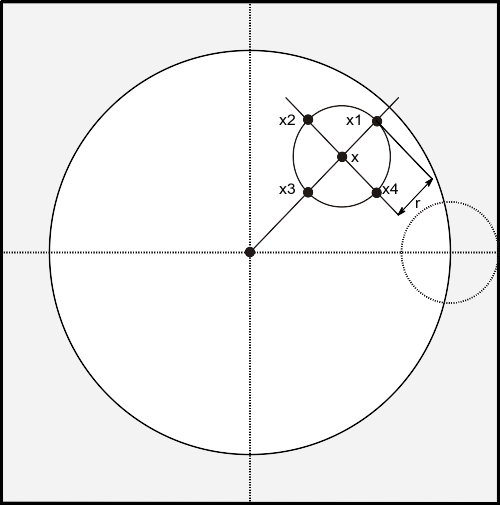
\includegraphics[width=7cm]{images/liop.png}
\caption{LIOP descriptor layout. courtesy: vlfeat.org}
\label{liop}
\end{figure}

Rotation invariant is achieved by taking neighbourhood pixels of pixel $x$ in the anticlockwise direction on a circle as shown in fig \ref{liop}. In order to develop  the histogram, the identified order of intensities in the neighbourhood  of pixels will map to a linear index. Bins are constructed based on the weighted pooling of mapped linear indices  in the region.

\begin{figure}[ht]
 \centering
 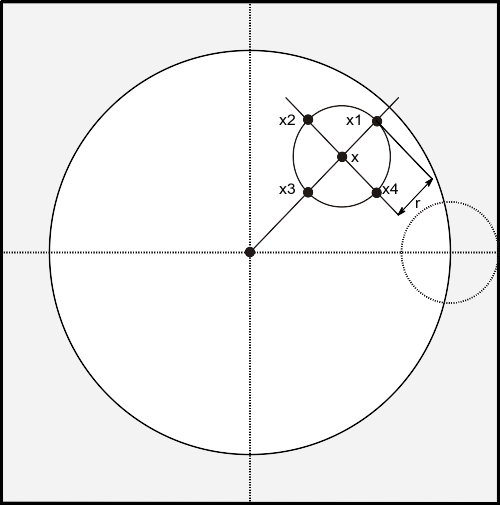
\includegraphics[width=7cm]{images/liop.png}
\caption{LIOP descriptor layout. courtesy: vlfeat.org}
\label{liop}
\end{figure}

\end{document}

